\documentclass{article}

\usepackage[utf8]{inputenc}

\usepackage{graphicx}
\usepackage{minted}
\usepackage[obeyspaces]{url}

\selectfont

\title{Konzept für Service-Manager}
\author{Christopher Mogler}
\date{April 2020}

\renewcommand*\contentsname{Inhalt}

\graphicspath{ {./img/} }

\begin{document}
\maketitle
\tableofcontents
\newpage

\section{SM.Database}

\subsection{Module}

Die Module sind in einer Datenbank-Tabelle hinterlegt. 
Die einzelnen Versionen sind in einer extra Tabelle hinterlegt.

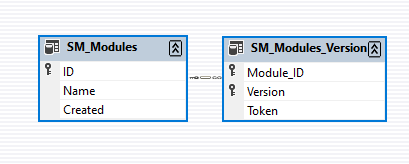
\includegraphics{db_modules}

\textbf{Modul-Tabelle}

\textbf{Versions-Tabelle}

Ein Satz besteht aus einer ID, Modul, Version, ein Datum wann es hinzugefügt wurde.
Jede Version bekommt einen eigenen Satz, jede Version bleibt erhalten.
\begin{itemize}
  \item \textbf{ID} ist pro Satz eindeutig besteht aus einer GUID.
  \item \textbf{Modul} zu welchem Modul diese Version zugehört. Es ist eine GUID die zur Modul-Tabelle verknüpft ist.
  \item \textbf{Version} welche Version es ist.
\end{itemize}
Die Anwendungen werden in einem bestimmten Verzeichnis aufbewahrt. Die Anwendungen werden pro Version abgelegt.
Bsp.: 
\path{/Anwendungen/MailInterface/1.14.1.zip}

\section{SM.API}

\subsection{Informationsabruf}

Um die Daten abzurufen muss sich die Schnittstelle authentifizieren. Dies erfolgt durch einen Token der für jeden Kunden einmalig ist.

\subsubsection{Datenaufbau}

Die Daten zum Abrufen der Informationen sind im JSON-Format. 
Bsp. wie die JSON-Datei aufgebaut ist:
\begin{minted}{json}
{
   "version": "1.0",
   "changed": "2020-04-02 12:12:12.222",
   "token": "50ad41624c25e493aa1dc7f4ab32bdc5a3b0b78ecc35b539936e3fea7c565af7",
   "modules": [
      {
         "id": "048e4a4e-ab6a-482e-9f34-8821325527f6",
         "name": "MailInterface",
         "version": "12.0.1",
         "token": "ad6af7308eab03163a9cbef49f22636efdb0f884620d777a29a8e8fc7634f967"
      },
   ]
}
\end{minted}

Erklärung: 
\begin{itemize}
  \item \textbf{version}: die aktuelle Version von Service-Manager.
  \item \textbf{changed}: letzte Änderung vom aktuellen Datensatz
  \item \textbf{token}: wird bei Änderungen verändert, damit die Schnittstelle schneller auf Änderungen prüfen kann. Ohne alle Module einzeln zu Prüfen.
  \item \textbf{modules}: alle Module die beim Kunden installiert sein muss.
  \begin{itemize}
  	\item \textbf{id}: ID vom Modul, wird verwendet um die Datei später herunterzuladen, über die API.
  	\item \textbf{name}: Name des Moduls
  	\item \textbf{version}: Aktuelle Version die Bereitgestellt wird.
  	\item \textbf{token}: Prüfungstoken um die installierte Version abzugleichen auf Änderungen.
  \end{itemize}
\end{itemize}

\subsection{Informationsänderung}

TODO

\newpage

\section{SM.Service}

\subsection{Ablauf}

Es wird eine Verbindung zur REST-API (siehe SM.Service) hergestellt. Die Informationen werden als JSON-Format übergeben.
Die Daten werden serialisiert in Objekte, damit die Verarbeitung vereinfacht wird.

\newpage

\section{SM.UI}

\subsection{Oberfläche}

TODO

\end{document}
